\chapter{PROCEDIMENTOS METODOLÓGICOS}
\label{chap:procedimentos-metodologicos}

Os procedimentos metodológicos definem as principais etapas realizadas para o desenvolvimento deste trabalho, incluindo as pesquisas, o desenvolvimento e avaliação do \textit{software}. Nas seções a 
seguir, descrevemos essas etapas.

\section{Definição do Processo}

Processos de \textit{software} são utilizados pelos engenheiros de \textit{software} para controlar e coordenar projetos de desenvolvimento de \textit{softwares} reais \cite{talma2006desenvolvimento}. 
\citeonline{padua2003engenharia} descreve um processo como um conjunto de passos parcialmente ordenados, constituídos por atividades, 
métodos, práticas e transformações, usados para atingir uma meta. 
Desta forma, um modelo de processo de \textit{software} é uma descrição simplificada de um processo, sendo também uma representação abstrata do mesmo para explicar as diferentes abordagens de 
desenvolvimento \cite{sommerville2003engenharia}. Tais processos de \textit{software} são complexos e dependem do julgamento humano como 
em qualquer processo intelectual. Sendo assim, não existe um processo de \textit{software} ideal, todos são desenvolvidos de maneiras 
diferentes por cada organização \cite{sommerville2003engenharia}.

O processo de \textit{software} utilizado para desenvolver o sistema foi baseado no modelo cascata, também chamado de ciclo de vida clássico, proposto por Royce em 1970. Neste modelo, as fases são 
sistematicamente seguidas de maneira sequencial \cite{pressman2006engenharia}. O modelo inicia com a fase de especificação de requisitos, passando pelo planejamento, modelagem, construção e 
implantação, finalizando na manutenção progressiva do software, como apresentamos na \autoref{fig:ciclo-cascata}.

As vantagens desse modelo se devem ao fato de que só se avança para a tarefa seguinte quando o cliente valida e aceita os produtos finais da tarefa atual, facilitando assim a compreensão adquirida ao 
longo do projeto, além de facilitar o processo de criação da documentação para o sistema \cite{pressman2006engenharia}. Já as principais desvantagens, segundo \citeonline{pressman2006engenharia}, se 
devem ao fato de que os projetos reais raramente seguem o fluxo sequencial ao qual o modelo propõe. Este modelo exige ainda que todos os requisitos sejam estabelecidos na fase 
inicial, fato que geralmente é difícil tanto para o cliente quanto para o desenvolvedor, pois os requisitos geralmente est\~ao em constante mudan\c{c}a. Outro grande problema com esse modelo é que o 
cliente só recebe uma versão executável do sistema no final de todo o processo de desenvolvimento, o que não agrada a muitos clientes.

Levando em consideração as vantagens e desvantagens antes citadas, esse modelo foi escolhido como base para o processo por facilitar o desenvolvimento de uma documentação mais detalhada e 
principalmente pela equipe de desenvolvimento ser formada por uma única pessoa, o autor deste trabalho, impossibilitando a divisão de tarefas característica de metodologias 
ágeis \footnote{Metodologias de desenvolvimento de software que tem enfoque nas pessoas e não em processos ou algoritmos, além de uma preocupação menor em documentação e maior em implementação 
\cite{michel2004metodologias}.}.

\begin{figure}[H]
    \centering
    \Caption{\label{fig:ciclo-cascata} Ciclo Cascata}	
    \UFCfig{}{
	\fbox{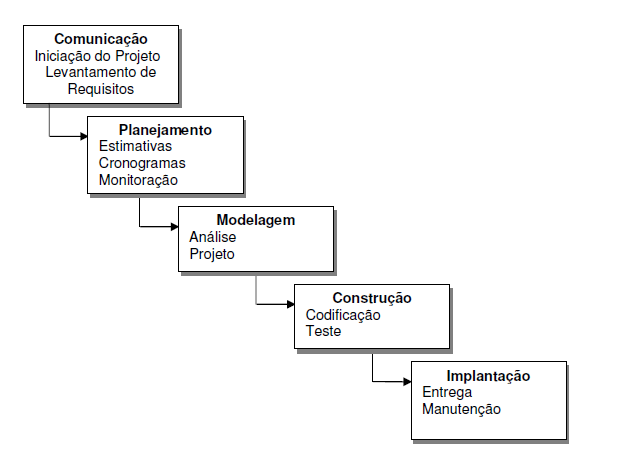
\includegraphics[width=7cm]{figuras/figura_ciclo_cascata}}
    }{
      \Fonte{\citeonline{pressman2006engenharia}}
    }	
\end{figure}


Dividimos o processo em nove atividades. A seguir, descreveremos brevemente cada uma delas:
\begin{alineascomnumero}
	\item \textbf{In\'icio do Projeto}: nessa atividade identificamos os objetivos do projeto e suas restri\c{c}\~oes.
	\item \textbf{Requisitos}: nessa atividade realizamos o levantamento e an\'alise dos requisitos, sua documenta\c{c}\~ao, verifica\c{c}\~ao e valida\c{c}\~ao, al\'em de um estudo para saber 
atrav\'es dos requisitos se o projeto \'e vi\'avel. 
	\item \textbf{Projeto}: nessa atividade desenvolvemos o projeto da arquitetura do sistema, o planejamento dos m\'odulos, o projeto da interface gr\'afica com o usu\'ario  e como ser\~ao 
persistidos as entidades do sistema.
	\item \textbf{Implementação}: nessa atividade escolhemos primeiramente um m\'odulo do sistema para implementar, em seguida planejamos como ocorrer\'a a implementa\c{c}\~ao desse 
m\'odulo, implementamos o m\'odulo, e por \'ultimo realizamos a integra\c{c}\~ao de m\'odulo ao resto do sistema. Esse ciclo \'e repetido at\'e que todos os m\'odulos estejam desenvolvidos.
	\item \textbf{Testes}: durante essa atividade realizaremos o planejamento dos testes para o sistema, em seguida executaremos os testes 
para cada m\'odulo do sistema e para o sistema como um todo, e por \'ultimo iremos gerar um relat\'orio com os resultados dos testes.
	\item \textbf{Implantação}: ap\'os o sistema desenvolvido e devidamente testado, ele segue para a implanta\c{c}\~ao, em que prepararemos 
a plataforma onde o sistema ser\'a executado e realizaremos a implanta\c{c}\~ao. Ap\'os a implanta\c{c}\~ao, realizaremos testes de 
aceita\c{c}\~ao e a cria\c{c}\~ao de um manual para o sistema.
	\item \textbf{Gerenciamento do Projeto}: essa atividade ocorre durante todo o desenvolvimento do sistema e tem por objetivo permitir que o projeto consiga ser conclu\'ido dentro do prazo e da 
qualidade desejada.
	\item \textbf{Avalia\c{c}\~ao do Processo}: essa atividade \'e executada durante todo o desenvolvimento do projeto e permite que o processo utilizado seja constantemente avaliado e adaptado 
conforme segue o desenvolvimento do projeto.
	\item \textbf{Encerramento do Projeto}: nessa \'ultima atividade ser\'a realizado apenas uma reuni\~ao em que ser\'a oficializado o final do projeto.
\end{alineascomnumero}

O processo desenvolvido est\'a dispon\'ivel em \url{www.askmath.quixada.ufc.br/static/process/}. 

\section{Levantamento e Análise de Requisitos}


O Levantamento e An\'alise de Requisitos é a fase do desenvolvimento de um \textit{software} em que o analista verifica junto ao usuário 
quais as necessidades, condições e princípios que o \textit{software} deverá atender \cite{matuda2013mapas}. Essa fase possibilitou 
conhecer e estudar as necessidades do cliente, assim como as restrições que o software estará sujeito.

Para realizar a coleta dos requisitos, optamos por utilizar entrevistas com o cliente, que no caso foi um dos professores de matemática da \gls{ufc}. Nessas entrevistas, que se caracterizaram como semi-estruturadas \footnote{Pois foram guiadas por um 
roteiro previamente elaborado e composto por questões abertas \cite{belei2008uso}}, foi possível obter os requisitos do sistema, assim como 
o público-alvo a quem o sistema atenderá. Essa técnica foi utilizada porque permitia uma organização flexível e ampliação dos 
questionamentos à medida que as informações foram sendo fornecidas pelo cliente \cite{fujisawa2000utilizaccao}.

A plataforma atender\'a quatro tipos de usu\'arios que formaram seu p\'ublico-alvo, ser\~ao administradores, professores, assistentes, e estudantes. Os administradores ser\~ao respons\'aveis por 
cadastrar novos professores, assim como realizar a manuten\c{c}\~ao do sistema. Os professores ser\~ao responsáveis por definir 
as disciplinas e li\c{c}\~oes que far\~ao parte do sistema. 
Ap\'os as disciplinas e li\c{c}\~oes serem definidas pelos professores, os assistentes ser\~ao respons\'aveis por manter\footnote{Adicionar, editar e excluir os problemas.} os problemas de cada 
li\c{c}\~ao. Os estudantes resolver\~ao os problemas desenvolvidos pelos assistentes e poder\~ao postar d\'uvidas sobre qualquer conte\'udo 
no f\'orum de discuss\~oes. Quando a plataforma for aplicado em sala de aula, os professores ser\~ao ainda respons\'aveis por gerenciar suas 
turmas e acompanhar o andamento do progresso de cada um de seus estudantes. J\'a os assistentes, ser\~ao responsáveis por tirar d\'uvidas 
dos estudantes no f\'orum de discuss\~oes.

Para uma melhor compreensão do público-alvo, foram criadas Personas \cite{pruitt2003personas}, personagens fictícios usados para 
caracterizar os papéis dos diferentes usuários do sistema \cite{guerra2010colaboraccao}. Cada Persona criada possui um nome, hábitos, 
histórias pessoais, motivações, objetivos, entre outras (ver \autoref{ap:personas}). A escolha dessa técnica deu-se pelo fato de que ela 
permite ao desenvolvedor saber mais precisamente para 
quem ele deveria construir o sistema, além de permitir uma distinção maior do público-alvo e, dessa forma, aprofundar-se nos interesses individuais de cada um.

Apresentaremos a seguir, os principais requisitos levantados durante essa etapa:

\begin{alineascomponto}
	\item Hierarquia dos Conteúdos: no sistema, dever\~ao existir disciplinas. Cada disciplina dever\'a possuir li\c{c}\~oes e cada li\c{c}\~ao ser\'a formada por problemas. Os professores poder\~ao 
cadastrar v\'arias disciplinas e li\c{c}\~oes, j\'a os assistentes ficar\~ao responsáveis por adicionar os problemas nas li\c{c}\~oes. Quando o estudante entrar no sistema, ele poder\'a ver somente 
as li\c{c}\~oes de uma disciplina por vez, podendo alternar entre disciplinas. Para um estudante come\c{c}ar a responder os problemas, ele dever\'a escolher inicialmente a disciplina e em seguida a 
li\c{c}\~ao. 

	\item Estrutura do Problema: cada problema possuir\'a uma descri\c{c}\~ao e v\'arios itens. Os problemas ser\~ao somente de m\'ultipla escolha e poder\~ao possuir no m\'inimo dois e no m\'aximo 
cinco itens. A quantidade de itens em cada problema ficar\'a a crit\'erio do assistente que adicionar\'a o problema ao sistema.

	\item Saltar Problemas: o sistema deverá permitir ao aluno saltar problemas e rever os saltos 
realizados com algumas restrições na quantidade de saltos..
	
	\item Pedir Ajuda: para todo problema, o estudante poderá consultar conte\'udo de ajuda. No momento em que o assistente estiver adicionando o problema, ele poderá ou não adicionar um texto de 
ajuda para o estudante, isso fica a critério dele. Quando o estudante estiver resolvendo os problemas, ele terá um botão que, quando acionado, mostrar\'a o texto de ajuda. O sistema dever\'a salvar a 
quantidade 
de vezes que o estudante pedir ajuda e em quais problemas.
	\item F\'orum: o sistema deverá possuir um fórum onde os estudantes possam postar suas dúvidas para que professores, assistentes e outro participantes possam lhes ajudar com o problema. Esse fórum, deve possuir tópicos, comentários para os tópicos, e os comentários devem oferecer a opção de se comentar com imagens.     

\end{alineascomponto}

Após o levantamento dos requisitos, foi realizada a análise dos mesmos. Nessa análise, os requisitos foram agrupados em categorias. As categorias utilizadas são descritas por 
\citeonline{sommerville2003engenharia} como:
\begin{alineascomponto}
    \item Requisitos Funcionais -- especificam ações que um sistema deve ser
capaz de executar, sem levar em consideração restrições físicas. Os requisitos
funcionais especificam, portanto, o comportamento de entrada e saída de um
sistema.
    \item Requisitos Não Funcionais -- descrevem apenas atributos do sistema ou
atributos do ambiente do sistema, como segurança, desempenho, usabilidade e
confiabilidade.
    \item Requisitos de Domínio -- são os requisitos do domínio da aplicação do sistema e que refletem características desse domínio.
\end{alineascomponto}

Após esse agrupamento, os requisitos funcionais foram representados em Casos de Uso \cite{jacobson92engenharia}. Um caso de uso identifica os agentes envolvidos em uma interação e especifica o tipo  de interação utilizando anotações sugeridas pela 
\gls{uml} \citeonline{sommerville2003engenharia}. Em seguida, foi realizada a documentação dos requisitos (ver \autoref{ap:requisitos}).

No final dessa etapa, ocorreu a Validação dos Requisitos junto ao cliente.  A Validação dos Requisitos é definida como o processo que certifica que o modelo de requisitos gerado  esteja  consistente  
com  as  necessidades  e  intenções  de  clientes  e usuários \cite{rilston2003metodologia}. Essa etapa permitiu que os requisitos coletados e documentados estivesse de acordo com o que o 
cliente solicitou.

\section{Projeto do Sistema}

O Projeto de Software é à atividade de engenharia cujo foco é definir ``como'' os requisitos estabelecidos no projeto devem ser implementados no software \cite{pressman2006engenharia}. O objetivo da  
atividade de projetar é gerar um modelo ou representação que apresente solidez, comodidade e deleite \cite{pressman2006engenharia}. Nesta fase, definimos como será aplicado o conhecimento obtido na 
pesquisa bibliográfica para se desenvolver o sistema. Para isto, definimos a arquitetura de software e as ferramentas que serão utilizadas durante o desenvolvimento do sistema. Nas seções a seguir, 
descrevemos um pouco sob cada um.

\subsection{Arquitetura}
Por arquitetura de software, entende-se a estrutura ou a organização de componentes de módulos, a maneira através da qual esses componentes interagem e a estrutura de dados que será usada pelos componentes \cite{pressman2006engenharia}.

A arquitetura utilizada baseia-se na arquitetura Cliente-Servidor\cite{david2013everything}, em que o processamento é dividido em processos distintos. Um processo é responsável pela manutenção da 
informação (servidor) e os outros são responsáveis pela captação de dados (clientes). Nessa arquitetura, os clientes enviam pedidos para o servidor, e este por sua vez processa estes dados e envia as 
respostas dos pedidos aos clientes.

Este modelo de arquitetura facilitará na manutenção do sistema, tendo em vista que toda atualização só necessitará ser realizada no servidor e automaticamente a mesma se propagará para todos os 
clientes. Com todos os recursos centralizados no servidor, podemos também ter um maior ganho com segurança, já que podemos centralizar os nossos esforços para manter a segurança das informações em 
apenas um único ponto, além de possibilitar que apenas cliente credenciados possam acessar e/ou alterar essas informações. Uma das outras grandes vantagens que temos  ao utilizar esse modelo, é que, 
\`a medida que a quantidade de clientes aumentar, será possível suprir esses clientes sem necessitar realizar nenhuma modificação essencial.

Para uma visualização mais detalhada da arquitetura de \textit{software} definida, ver o  \autoref{ap:arquitetura}.

\subsection{Ferramentas}

A análise do sistema foi feita com o auxílio da ferramenta de criação de diagramas Astah \cite{astah2016}. A implementação com a linguagem 
Python \cite{vanrossum2010python}, o sistema de gerenciamento de banco de dados PostgresSQl \cite{momjian2001postgresql} e a camada de 
aplicação utilizar\'a o framework Django \cite{django2016}. O módulo Rosseta \cite{rosetta2016} ser\'a empregado 
para permitir a internacionalização do sistema.
 
A seguir, apresentaremos a lista das ferramentas e das tecnologias utilizadas para o desenvolvimento do projeto:

\begin{alineas}
	\item \textbf{Astah}: para a modelagem baseada em \acrshort{uml} do sistema.
	\item \textbf{Python}: linguagem de programação para implementação do sistema.
    \item \textbf{Django}: framework web responsável pela camada de aplicação.
    \item \textbf{Rosetta}: aplicação desenvolvida em Django que facilitará a tradução do projeto para diversas línguas.  
    \item \textbf{PostgreSQL}: como banco de dados para armazenamento e consulta de informações.
    \item \textbf{Metro UI CSS}: framework que faz uso de HTML, Cascading Stype Sheet (CSS) e Javascript para criação do front-end do sistema.
    \item \textbf{MathJax}: \'e uma engine\footnote{Uma biblioteca ou pacote de funcionalidades que são utilizadas para facilitar o desenvolvimento de alguma tecnologia.} de código aberto 
desenvolvido em 
javascript na forma de um plugin para incluir equações matemáticas em todos os navegadores, esse plugin aceita expressões em  MathML e Latex.

\end{alineas}

Algumas dessas ferramentas foram selecionadas por se tratarem de ferramentas \textit{Open Source}, ou seja, que seu código-fonte pode ser 
alterado para diferentes fins, possibilitando assim que qualquer um consulte, examine ou as modifique, e outras por serem ferramentas que 
possibilitam um rápido desenvolvimento.

No final dessa etapa, foi gerado o Plano de Projeto, documento que guiou o desenvolvedor durante todo o processo de desenvolvimento.

\section{Implementação do Sistema}

A implementação envolve as atividades de codificação, compilação e integração. A codificação visa traduzir o design num programa, utilizando linguagens e  ferramentas adequadas. A codificação 
deve refletir a estrutura e o comportamento descrito no projeto. Os componentes arquiteturais devem ser codificados de forma independente e depois integrados \cite{aguiar2012requisitos}.

O ambiente de desenvolvimento que est\'a sendo utilizado para desenvolver o sistema consiste em:
\begin{alineas}
	\item \textbf{Sistema Operacional}: Ubuntu 14.04 LTS;
	\item \textbf{Interpretador}: Python 2.7.6;
	\item \textbf{Banco de Dados}: PostgreSQL 9.3.13;
	\item \textbf{\textit{Framework} de \textit{back-end}}: Django 1.7.11;
	\item \textbf{\textit{Framework} de \textit{front-end}}: Metro UI CSS 3.0.15;
\end{alineas}

Para permitir uma maior independ\^encia desse ambiente com a maquina em que estamos desenvolvendo o sistema, decidimos criar um ambiente de desenvolvimento com o auxilio da 
ferramenta Virtualenv 15.0.2. O Virtualenv permite isolar o ambiente de desenvolvimento de um determinado projeto para garantir que um pacote instalado não interfira nos demais projetos que 
rodam na maquina, al\'em de possibilitar saber facilmente a vers\~ao de todos os pacotes e componentes que est\~ao sendo utilizados para desenvolver o sistema. Essa informa\c{c}\~ao \'e 
importante quando formos replicar o ambiente de desenvolvimento no servidor de produ\c{c}\~ao\footnote{O ambiente de produção é onde os usuários finais acessarão o software}. 

Todos os c\'odigos-fonte gerados nessa etapa, passaram por um processo de versionamento\footnote{O versionamento de uma aplicação tem como 
foco principal documentar as inclusões, alterações ou até mesmo exclusões de funcionalidades.} atrav\'es da ferramenta Git 1.9.1, 
essa ferramenta permite:

\begin{alineascomponto}
	\item \textbf{Controle do histórico}: facilidade em desfazer e analisar o histórico do desenvolvimento, como também facilidade no resgate de versões mais antigas e estáveis.
	\item \textbf{Marca\c{c}\~ao e Resgate de Vers\~oes Est\'aveis}: permite marca onde um documento estava com uma vers\~ao est\'avel, para ser facilmente resgatado no futuro.
	\item \textbf{Ramifica\c{c}\~ao do Projeto}: permite dividir o projeto em v\'arias linhas de desenvolvimento sem que uma interfira na outra. 
\end{alineascomponto}

No final dessa etapa, tivemos os códigos-fonte de todos os módulos do sistema, assim como o próprio sistema em funcionamento. 

\section{Verificação e Validação}
Essa etapa destinou-se a mostrar que o sistema está de acordo com a especificação e que ele atende às expectativas de clientes e usuários, al\'em de assegurar que o  programa está fazendo aquilo que foi definido na sua especificação e que não possui  erros  de execução \cite{aguiar2012requisitos}. 

Durante essa fase, realizamos Testes de Unidade e Integra\c{c}\~ao em cada modulo do sistema, assim como Testes de Sistema no sistema j\'a integrado.

\citeonline{aniche2014teste} define essas categorias de Testes de Software como:

\begin{alineascomponto}
	\item \textbf{Teste de Unidade} -- é aquele que testa uma única unidade do sistema. Ele a testa de maneira isolada, geralmente simulando as 
prováveis dependências que aquela unidade tem. Em sistemas orientados a objetos, é comum que a unidade seja uma classe. Ou seja, quando 
queremos escrever testes de unidade para a classe Pedido, essa bateria de testes testará o funcionamento da classe Pedido, 
isolada, sem interações com outras classes.
	\item \textbf{Teste de Integração} -- é aquele que testa a integração entre duas partes do seu sistema. Os testes que você escreve para a sua 
classe PedidoDao, por exemplo, em que seu teste vai até o banco de dados, é um teste de integração. Afinal, você está testando a integração 
do seu sistema com o sistema externo, que é o banco de dados. Testes que garantem que suas classes comunicam-se bem 
com serviços web, escrevem arquivos texto, ou mesmo mandam mensagens via \textit{socket} são considerados testes de integração.
	\item \textbf{Teste de Sistema} -- \'e aquele que garante que o sistema funciona como um todo. Este 
nível de teste está interessado se o sistema funciona como um todo, com todas as 
unidades trabalhando juntas. Ele é comumente chamado de teste de caixa preta, já 
que durante o teste n\~ao se importa com a forma que os dados s\~ao processados, mas sim se as sa\'idas est\~ao de acordo com o que era esperado para entradas. 
\end{alineascomponto}

\section{Definição dos Conteúdo para o Sistema}

Após o sistema estar verificado e validado, tivemos que adicionar conteúdos para serem utilizados por usu\'arios durante os testes da \textit{interface}. Decidimos optar por deixar os monitores\footnote{É o aluno de graduação concursado para exercer, juntamente com o professor, atividades técnico-didáticas condizentes com o seu grau de conhecimento junto à determinada disciplina, já por ele cursada.} das turmas de matemática desenvolverem os conteúdos que foram utilizados no sistema durante a fase de avaliação. 

Os monitores passaram por um treinamento, no qual aprenderam a utilizar o sistema para adicionarem os conteúdos.